\clearpage
\section{Prototype Implementation}
\label{sec:implementation}

\subsection{Frontend}
The following components have been implemented for the front end:

\begin{itemize}
	\item Login: this is the first view that the user are presented with. It’s main purpose is to
authenticate users, and help them access the application. It contains input fields for
username and password. When the user presses “Log in”, he is taken to the main-page of the
application. If the user is not registered, he can easily do so by pressing the “Register”-
button.
	\item Register: here the user is presented a schema, where he can register and that way access the
application. He needs to add an email address, a username and a password. Once the
information is submitted, the user is sent back to the login page.
	\item Main-page: This component contains buttons that lets the user easily navigate to all parts of
the application quickly.
	\item Find-poll: Here the user can search for a poll via its id, or by a poll-name. All the polls that
matches the input will then be displayed with the option to vote on it.
	\item Create-poll: Here the user can create a new poll. He can decide the questions that should be
displayed, when the poll is active, if it is private and invite users to participate in it. Once
created, a poll-id is given to the user. This can for example be given to other users and used
to search for the poll.
	\item Vote: Here the user gets to submit votes to active polls.
\end{itemize}

\noindent A authentication service, a poll service and a voting service has also been created to handle logic that
can be applied to multiple components. The authentication service handles operations such as
logging the user in to the application and searching for users. The poll service handles logic depicting
the polls such as finding polls, creating polls and changing polls. The Voting service handles the logic
connected to the voting.  The following subsection describes more detailed how the logic behind the authentification process has been implemented, 
and displays how the frontend is connected to the REST API. 

\subsubsection{Authentication Process}
A crucial part of the frontend implementation is the user authentication process. 
This is managed through the \texttt{login} method in the \texttt{auth.service} file and the \texttt{onSubmit} method in the \texttt{LoginComponent}.  The \texttt{login} method is defined as: \\

\begin{center}
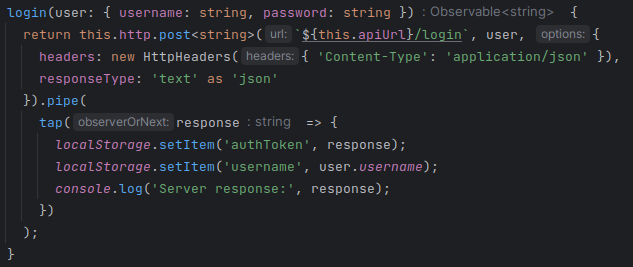
\includegraphics[width=0.80\textwidth]{figs/login.png}
\end{center}

\noindent This method handles user login credentials, sending them to the backend for verification and storing the received token and 
username in the browser's local storage for session management. The token is stored in the local storage to maintain the user sessions. \\

\noindent The \texttt{LoginComponent} uses this service in its \texttt{onSubmit} method: \\

\begin{figure}[h]
  \centering
  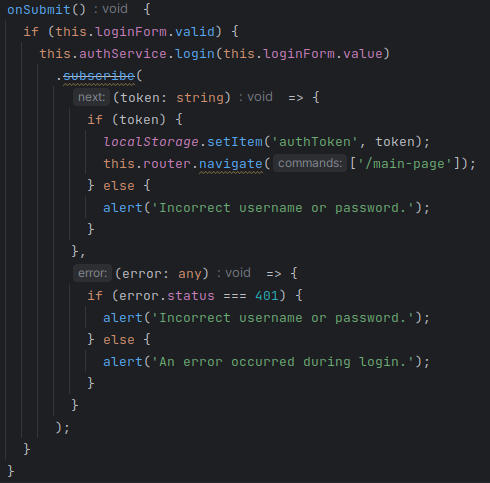
\includegraphics[width=0.80\textwidth]{figs/on_submit.png}
  \caption{Verification Service Example}
  \label{fig:my_label}
\end{figure}

\noindent This function makes sure that only users with valid credentials are able to access the main page of the application, while also handling 
different error scenarios. If a user gives an incorrect credential or any other login error occurs, an error message is displayed. \\

\subsection{Backend}
The architecture of our program has modular architecture that includes multiple important entities and their corresponding repositories.

\subsubsection{Entities}
We will begin by describing the structural components of the application which is object-oriented by design. The primary class, \texttt{AppUser}, implements properties such as username, email, and password. It also holds a collection of polls owned by the AppUser.  A critical feature of this class is the implementation of two-factor authentication, validated through a verification code to ascertain user authenticity. \\

\noindent The \texttt{Poll} class, a core entity in our application, represents polls created by users. It includes details like title, open/close status, and duration, and can contain multiple questions. The poll implements general properties for storing privacy status, activity status, duration, and IoT device pairing. It also implements specific properties like the poll title, vote tallies, a list of authorized users (for private polls only) and funttion implementation to perform question management such as add, delete and edit. Polls are also linked to IoT device and therefore, holds information on which device it is paired with.\\

\noindent The \texttt{Question} class constitutes individual items within polls for users to vote on. Records responses and associates with specific polls.\\

\noindent A \texttt{Vote} class records user votes in polls, indicating 'yes' or 'no' choices. It contains the logic that is responsble for determining which question in a poll the vote should be submitted towards.\\

\noindent The \texttt{IoTDisplay} is a singleton class only aware of its associated IoT device by the property pariedDevice, which contains a string value of of the device name. \\

\noindent \texttt{ThirdPartyApp} interface class provides logic to allow third party entties to retreive data from the application. \\


\subsubsection{Repositories}
JPA repositories helps with performing create, read,update and delete (CRUD) database operations by reducing the need to manually code complex SQL queries.  We use these repositories with JPA EntityManager to interact with the database. We have defined various repositories in the FeedApp responsible for handling specific data operations.\\

\noindent The \texttt{AppUserRepository} manages the \texttt{AppUser}entity data operations, including user lookup by username.
\noindent \texttt{PollRepository} handles data operations for the \texttt{Poll} entity, with custom queries for poll title searches.\\

\begin{figure}[h]
  \centering
  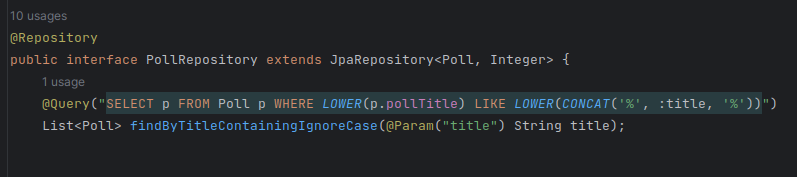
\includegraphics[width=0.80\textwidth]{figs/poll_repository.png}
  \caption{Custom Poll Title Query}
  \label{fig:my_label}
\end{figure}

\noindent The \texttt{QuestionRepository} provides data access for \texttt{Question} entity.
\noindent \texttt {VoteRepository} manages \texttt{Vote} data, including vote counting in polls.

\begin{figure}[h]
  \centering
  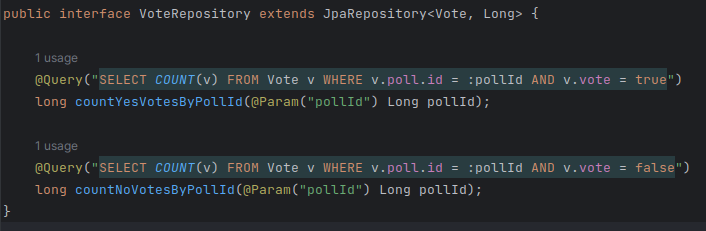
\includegraphics[width=0.80\textwidth]{figs/vote_repository.png}
  \caption{CustomVoting Query}
  \label{fig:my_label}
\end{figure}

\subsubsection{Integration with Spring Boot, Hibernate, and JPA}
Our voting application uses:

\begin{itemize}
    \item {Spring Boot} as a framework, simplifing configuration and setup.
    \item {Hibernate} as the ORM tool, translating Java objects to database representations.
    \item {JPA interfaces}, such as \texttt{JpaRepository}, for efficient data access and manipulation.
\end{itemize}

\subsubsection{Functionality}

Supported data models functionalities in our application:
\begin{itemize}
    \item User registration and management.
    \item Interactive poll creation and management.
    \item Voting mechanisms within polls.
    \item Integration with IoT devices for an enhanced user experience.
\end{itemize}

\subsection{REST API}
The web application consists of three key controllers, each handling different aspects of the voting system:

\begin{itemize}
    \item The AppUserController is responsible for user-related functions, including user authentication, registration, and the verification process.  It implements the AppUser entity using depencency injection by the @Autowired annotation to reference AppUserRepository and AppUserService. 
    \item The PollController oversees the management of polls, specifically handling the publication of poll results and controlling their status, whether open or closed.
    \item The QuestionController introduces and manages a voting mechanism for individual questions, reflecting a finer level of interaction and user engagement within the application.  It is mapped 
    \item The IOTController class in annotated with @RestController which is part of a RESTful web service in a Java application using the Spring Framework. It handles HTTP requests specifically related to IoT device notifications.  The controller is mapped to handle requests at the /api/notifications path.  It defines two endpoints for processing notifications sent from the IoT device, /api/notification/greenVote and /api/notification/redVote.  
\end{itemize}

\begin{figure}[h]
  \centering
  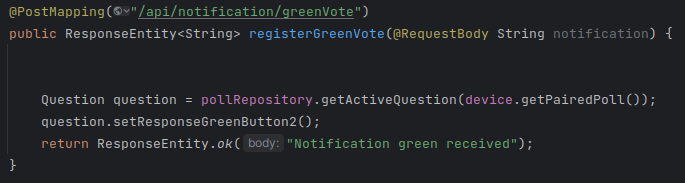
\includegraphics[width=0.80\textwidth]{figs/green_vote.png}
  \caption{Green Vote Endpoint}
  \label{fig:my_label}
\end{figure}

\noindent All controllers are designed following REST principles, offering a specific base URLs and using HTTP methods for standard CRUD operations.

\subsubsection{Spring Boot and Spring Data Integration}
They utilize Spring Boot's capabilities for creating standalone applications and Spring Data's repository pattern for data access. Dependency injection with \texttt{@Autowired} is also used.

\subsubsection{Error Handling and Response Management}
The controllers use \texttt{ResponseEntity} class for HTTP response handling, allowing them to manage different scenarios (even those ending with an error).  Method \texttt{deleteQuestion} in \texttt{QuestionController} that is responsible for deleting a question in a poll returns an error response if the question wasn't found:

\begin{figure}[h]
  \centering
  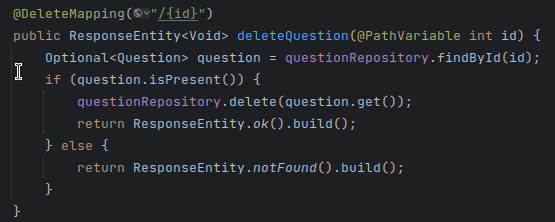
\includegraphics[width=0.80\textwidth]{figs/delete_mapping.png}
  \caption{Error Handling Response}
  \label{fig:my_label}
\end{figure}


\subsubsection{Security and User Management}
The \texttt{AppUserController} focuses on security and user identity management through authentication and JWT token management.  There are also a few features that we modelled into our application in the first phase of this project,
but due to the time constraints are yet to be implemented. These include Poll management and User
management. Currently the application allows users to create and participate in polls. However, the
management of the polls is not yet functional. The same goes for the management of the user
settings. The buttons has been created in the main-page component, but they are not directing the
users to new views yet.

\subsubsection{IoT Device}
The IoT device in our system, a physical unit, is implemented using C++ and is based on the ESP 8266 module, enabling Wi-Fi connectivity. This device is programmed with hardcoded Wi-Fi credentials which in our case is a cellar hotspot. Its design is straightforward, featuring just two buttons, referred to as the red and green buttons. The device is configured to publish a message to the MQTT broker whenever a button is pressed; however, it does not register continuous presses but only single clicks. These messages are then relayed by the MQTT broker, post distinct messages via REST interfacing with the IoTController.

  \begin{center}
  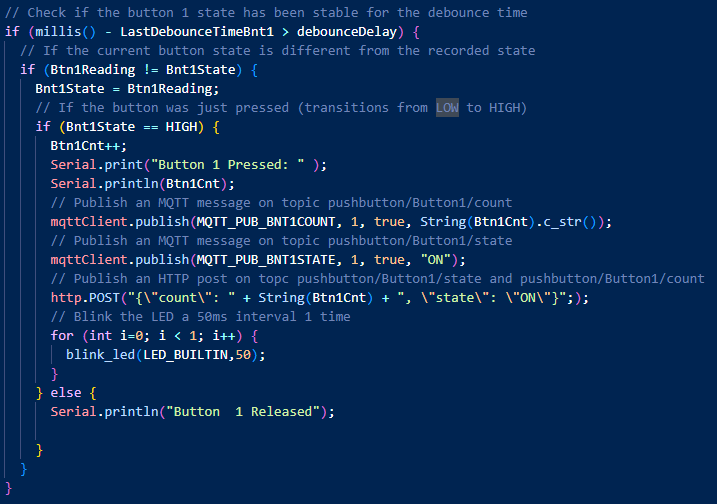
\includegraphics[width=0.80\textwidth]{figs/button1_pressed.png}
  \end{center}

